\documentclass{article}
\usepackage[margin=2.5cm, top=4cm, headheight=25pt]{geometry}
\usepackage{amsmath, amssymb, enumitem, fancyhdr, graphicx}
\usepackage[indent=20pt]{parskip}
\usepackage[hidelinks]{hyperref}
\usepackage{xcolor}
\usepackage{listings}
\usepackage{subcaption}
\usepackage{url}
\usepackage[most]{tcolorbox}
\usepackage{lastpage}

\tcbuselibrary{listingsutf8} % Support for lstlistings within tcolorbox

\newtcolorbox[auto counter, number within=section]{question}[1][]{%
    colframe=gray!80,                      % Dark gray frame
    colback=gray!5,                       % Light gray background
    coltitle=black,                        % Black title
    title=\textbf{Question~\thetcbcounter}, % Bold title
    fonttitle=\bfseries\large,             % Subtle title font size
    rounded corners,                   % Slightly more rounded corners
    boxrule=0.25mm,                         % Thinner border for a sleek look
    enhanced,                              % Enhanced box features
    attach boxed title to top left={xshift=2mm, yshift=-2mm},
    boxed title style={colframe=gray!80, colback=gray!5, boxrule=0.25mm},
    % Title styling
    #1
}

\bibliographystyle{IEEEtran}
\graphicspath{{./images/}}

% -- Custom Variables --
\def\me{Rajdeep Gill (7934493)}
\def\partner{Daniyal Hasnain (7942244)}
\def\course{ECE 4830}
\def\labsection{B03}
\def\labno{3}
\def\title{Lab 3}

% -- Styling for code snippets --
\lstset{
    basicstyle=\ttfamily\small,           % Basic font style
    keywordstyle=\color{blue},            % Keywords color
    commentstyle=\color{gray},            % Comments color
    stringstyle=\color{teal},             % Strings color
    numbers=left,                         % Line numbers on the left
    numberstyle=\tiny\color{gray},        % Line number style
    stepnumber=1,                         % Line number step
    numbersep=10pt,                       % Space between line numbers and code
    backgroundcolor=\color{lightgray!10}, % Background color
    frame=single,                         % Adds a frame around the code
    breaklines=true,                      % Line breaking for long lines
    captionpos=b,                         % Caption position
    showspaces=false,                     % Don't show spaces
    showstringspaces=false                % Don't show spaces in strings
}
\renewcommand{\lstlistingname}{Code Snippet}

\renewcommand{\arraystretch}{1.2} % For less-ugly tables
\setlength\parindent{0pt}

%----- Samples 
% Questions:
%   \begin{question}[title=Custom Question Title]
%       Question details
%   \end{question}

% Tables:
%   \begin{table}[htbp]
%       \centering
%       \caption{Table Caption}
%       \begin{tabular}{ll}
%           \toprule
%           \textbf{Column 1} & \textbf{Column 2} \\
%           \midrule
%           Row 1 & Row 2 \\
%           Row 3 & Row 4 \\
%           \bottomrule
%       \end{tabular}
%   \end{table} 

% Figures:
%   Single figure:
%       \begin{figure}[htbp]
%           \centering
%           \includegraphics[width=0.5\textwidth]{example-image}
%           \caption{Figure Caption}
%       \end{figure}
%   Multiple figures:
%       \begin{figure}[htbp]
%           \centering
%           \begin{subfigure}[b]{0.5\textwidth}
%               \includegraphics[width=\textwidth]{example-image-a}
%               \caption{First subfigure}
%           \end{subfigure}
%           \begin{subfigure}[b]{0.5\textwidth}
%               \includegraphics[width=\textwidth]{example-image-b}
%               \caption{Second subfigure}
%           \end{subfigure}
%           \caption{Main figure}
%       \end{figure}

\begin{document}

% --------------------------------------------------------------------------------
% TITLE
% --------------------------------------------------------------------------------

\begin{center}
    \huge \title

    \vspace{2mm}
    \hrule

    \vspace{4mm}
    \large \me ~\&~\partner

    \vspace{2mm}
    \large \course~\labsection

    \vspace{2mm}
    \today
\end{center}

\vspace{4mm}

% --------------------------------------------------------------------------------
% END TITLE
% --------------------------------------------------------------------------------

\newpage

\tableofcontents

\vspace{1cm}
\newpage

\pagestyle{fancy}
\fancyhead[L]{\large Lab \labno}
\fancyhead[R]{\large \me, \partner}

\fancyfoot[C]{Page \thepage~of~\pageref{LastPage}}

% --------------------------------------------------------------------------------
% BODY
% --------------------------------------------------------------------------------

\section{Problem 1}

a) To effectively use the Fourier Transform to classify each sound as Gear 1 or 2, we can work with the decibel scale because it factors in volume changes; any volume change will only shift the output up or down, maintaining all proportions otherwise. In other words, we plot the magnitude in dB of the two \textit{FFTs}, and distinguish distinct properties of the two gears.

The plot below shows the \textit{FFT} of the given gear examples:

\begin{figure}[h]
    \centering
    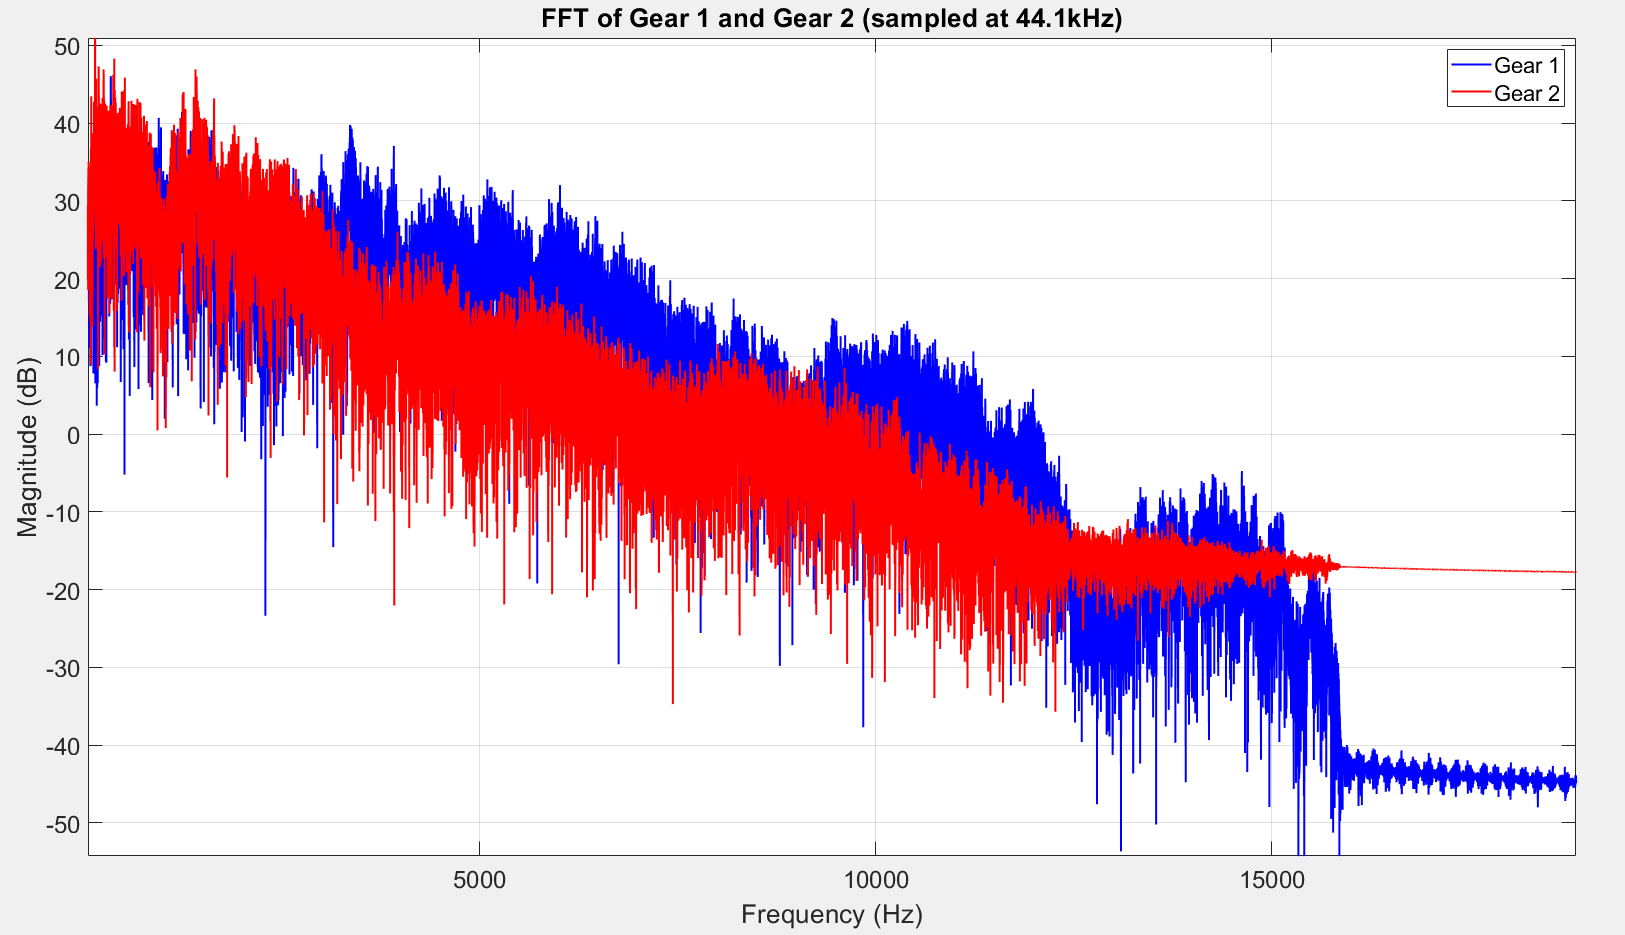
\includegraphics[width=0.75\textwidth]{FFT in dB (44.1kHz).png}
    \caption{The FFT of gear 1 and 2 in decibels, sampling at 44.1kHz.}
    \label{fig:fft_44.1kHz}
\end{figure}

The above plot shows a similar trend for both gears from 0 to 10kHz: both gears start at most at 50 dB and steadily decline with noticeable overlap. The primary distinguishing factor is the band running from 10kHz to 15kHz. Here, we see that gear 2 continues to decline, plateauing to -20 dB, whereas gear 1 has a decaying oscillation-like behaviour that strongly differs from gear 2. With this in mind, our technique involves \textbf{using a band-pass filter that attenuates all frequencies outside the 10k-15kHz range}, focusing the observed behaviour for classification.

\vspace{1cm}

b) Yes, we can reduce the sampling rate and not use \( F_s = 40000\) Hz. Based on the band-pass proposed in part (a), we suggest a sampling frequency that satisfies the Nyquist Criterion. To retain all key information, we set:

\[
F_{\text{max}} = 15000 \text{ Hz} \implies F_s \geq 2 \times 15000 = 30000 \text{ Hz}
\]

To provide a safer margin and ensure no aliasing effects, we choose:

\[
F_s = 32000 \text{ Hz} = \textbf{32 kHz}
\]

This sampling rate effectively captures all relevant frequencies based on the solution developed in part (a). 

We now proceed to plot the \textit{FFT} of both examples once more, this time, sampling at our suggested frequency:

\begin{figure}[h]
    \centering
    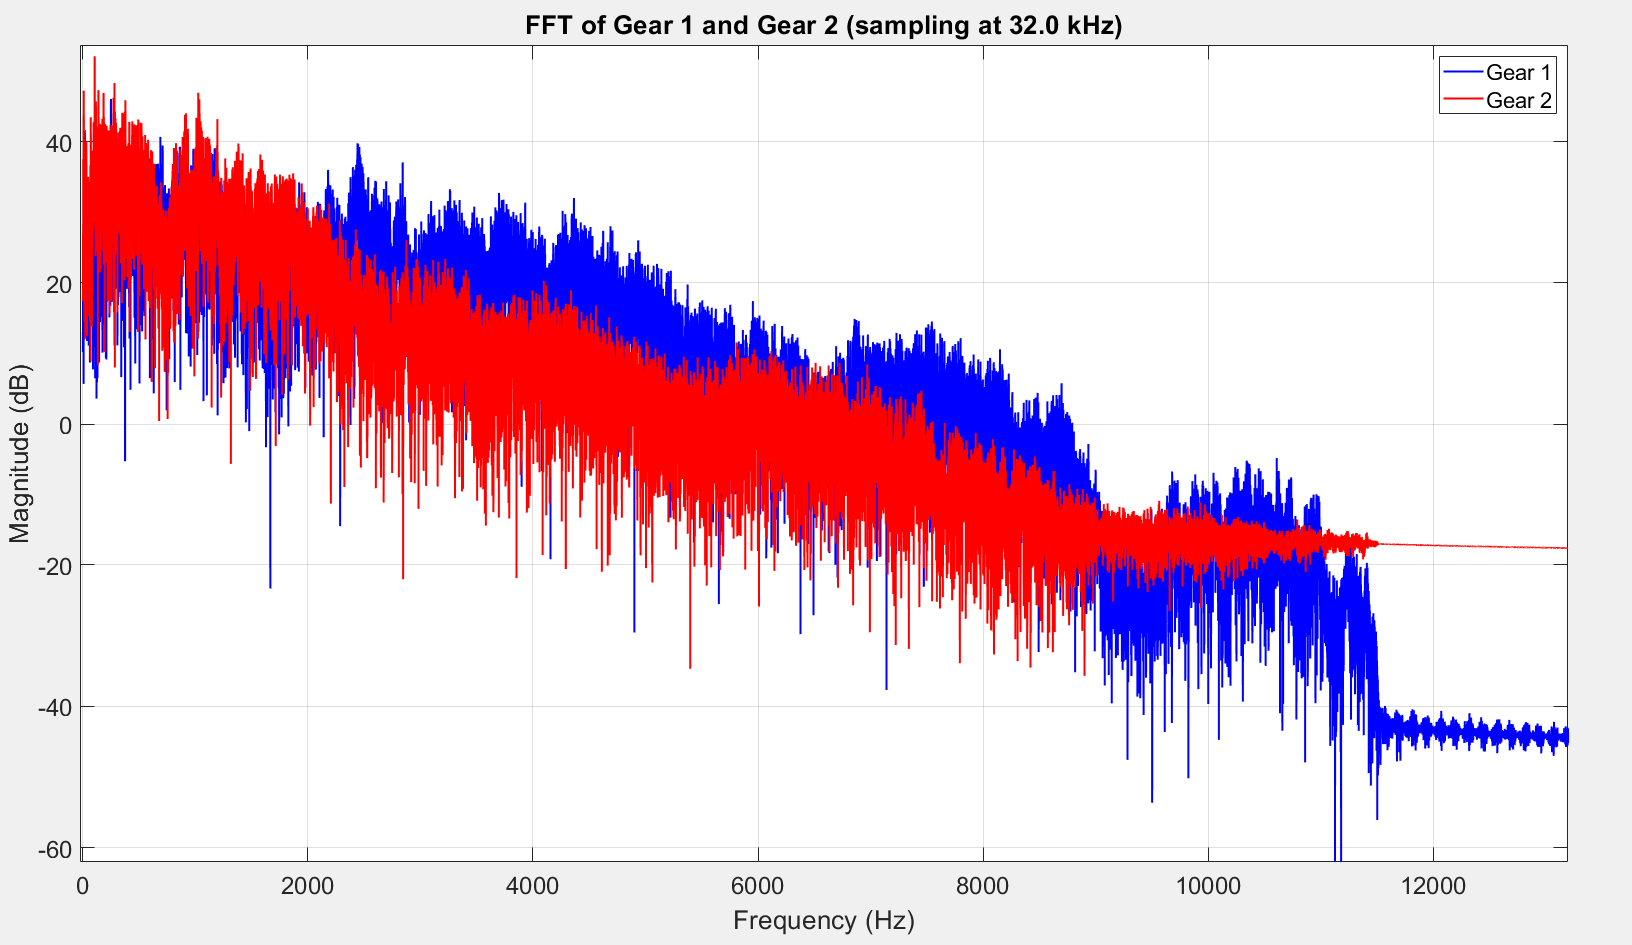
\includegraphics[width=0.5\textwidth]{FFT in dB (32kHz).png}
    \caption{The FFT of gear 1 and 2 in decibels, sampling at 32kHz.}
    \label{fig:enter-label}
\end{figure}

As expected, we see the same output based on our plot in part (a) but with a left shift in the frequency axis. Due to this horizontal shift, \textbf{we must also shift our band-pass to the 6k-11kHz range}  which can be done by altering the impedance and capacitance of the RLC circuit. This is the only change we need to implement in order to use the solution from part (a).

\section{Problem 2}
Plotting out the frequency spectra for the first unltrasound scan from samples 0 to 200 and then its subsequent echos from samples 201 to 800, we see the following results.

\begin{figure}[ht!]
    \centering
    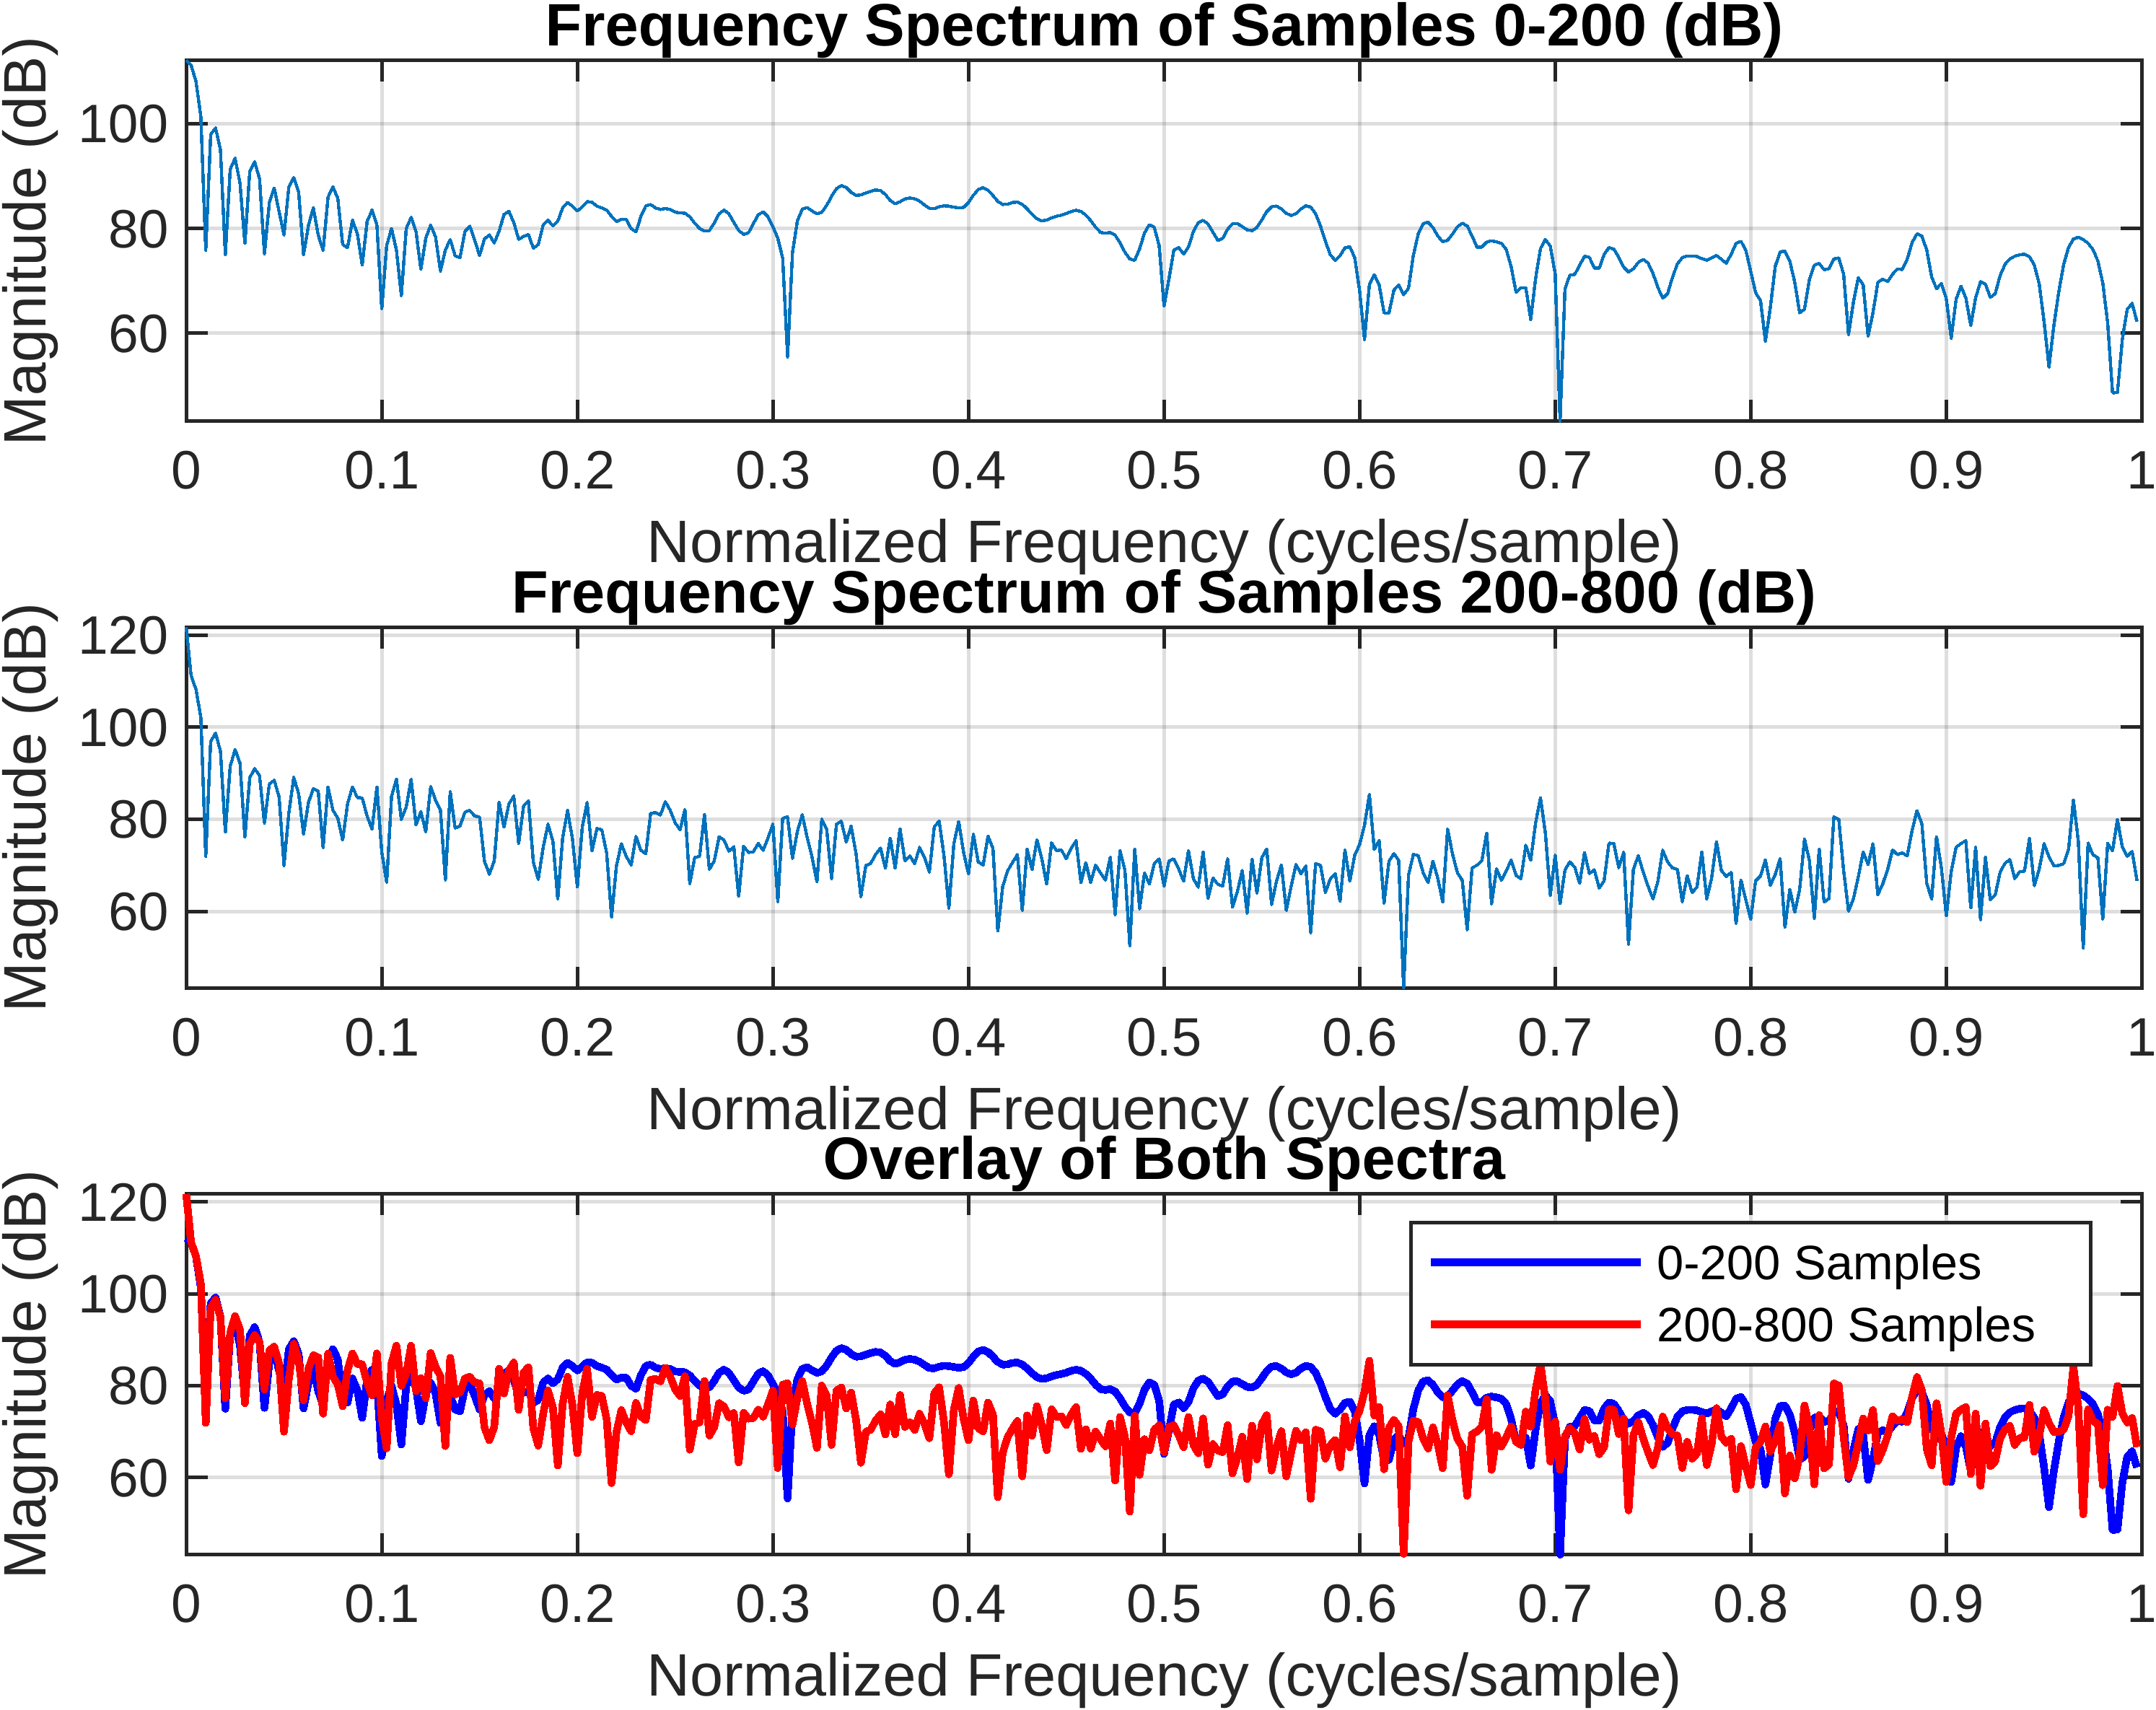
\includegraphics[width=0.5\textwidth]{p2_1.png}
    \caption{Frequency spectra of the first scan and echos}
\end{figure}

Since we are not given a sample time, or sampling frequency, we range our frequency axis from 0 to 1. We can then see that between 0.3 and 0.7 we have a difference between the first scan and the echos. Filtering this using a band pass filter will allow us to mitigate the echos and only focus on the first scan.

This will also remove the DC term, so we can re-add the average of the first scan to the filtered signal to get the desired output.

Below we can see the signal before and after filtering:
\begin{figure}[ht!]
    \centering
    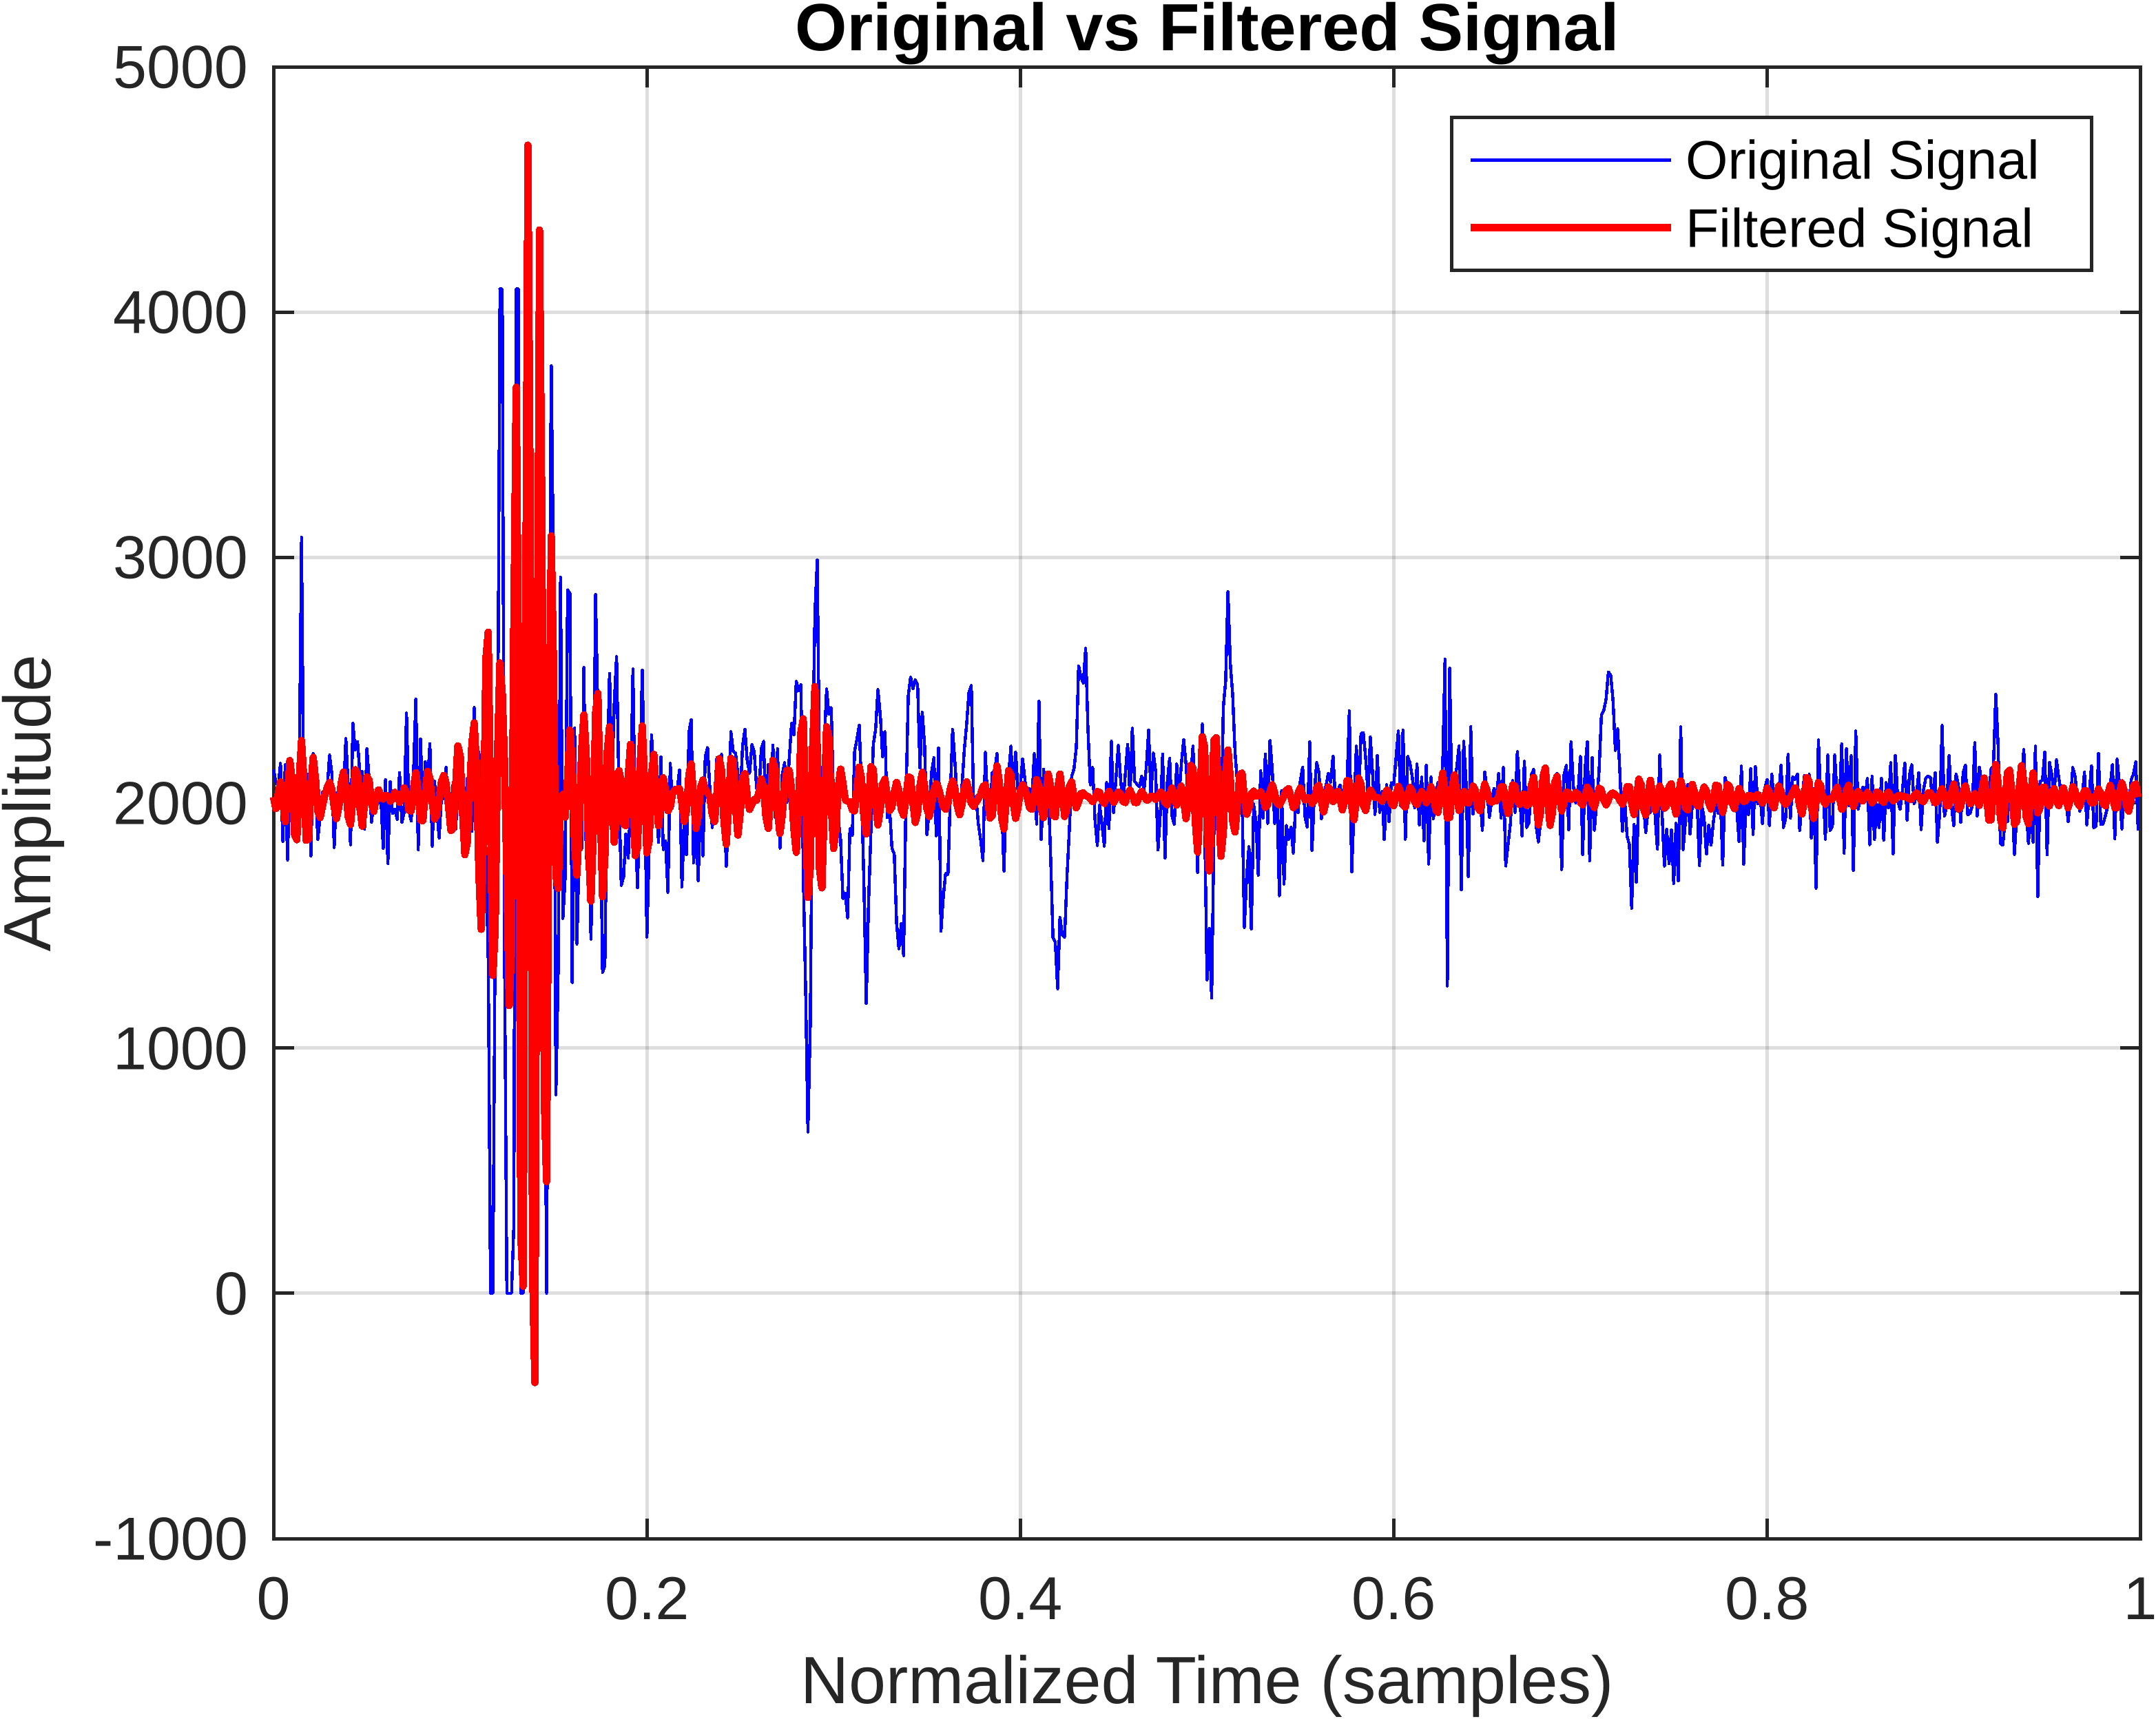
\includegraphics[width=0.5\textwidth]{p2_2.png}
    \caption{Signal before and after filtering}
\end{figure}
\section{Problem 3}

The given fourier transform is a triangular function defined as follows:
\begin{align*}
    X(\omega) &= \begin{cases}
        1 + \frac{4}{\pi} \omega & \text{if } -\frac{\pi}{4} \leq \omega \leq 0 \\
        1 - \frac{4}{\pi} \omega & \text{if } 0 \leq \omega \leq \frac{\pi}{4} \\
    \end{cases}
\end{align*}

Using the differentiation property:
\begin{align*}
    nx(n) \leftrightarrow j \frac{dX(\omega)}{d\omega}
\end{align*}

The derivative of the given triangular function is:
\begin{align*}
    \frac{dX(\omega)}{d\omega} &= \begin{cases}
        \frac{4}{\pi} & \text{if } -\frac{\pi}{4} \leq \omega \leq 0 \\
        -\frac{4}{\pi} & \text{if } 0 \leq \omega \leq \frac{\pi}{4} \\
    \end{cases}
\end{align*}

The inverse fourier transform of the derivative is:
\begin{align*}
    nx(n) &= j \frac{1}{2\pi} \int_{-\pi}^{\pi} \frac{dX(\omega)}{d\omega} e^{j \omega n} d\omega \\
    &= j \frac{1}{2\pi}\int_{-\frac{\pi}{4}}^{0} \frac{4}{\pi} e^{j \omega n} d\omega + j \int_{0}^{\frac{\pi}{4}} -\frac{4}{\pi} e^{j \omega n} d\omega \\
    &= j \frac{1}{2\pi}\left[ \frac{4}{\pi jn} e^{j \omega n} \right]_{-\frac{\pi}{4}}^{0} - j \left[ \frac{4}{\pi jn} e^{j \omega n} \right]_{0}^{\frac{\pi}{4}} \\
    &= \frac{2}{\pi^2 n} \left[ \left(e^{j\omega n}\right)\Bigg|_{-\frac{\pi}{4}}^{0} - \left(e^{j\omega n}\right)\Bigg|_{0}^{\frac{\pi}{4}} \right] \\
    nx(n) &= \frac{2}{\pi^2 n} \left[ 1 - e^{-j\frac{\pi}{4} n} - e^{j\frac{\pi}{4} n} + 1 \right] \\
    x(n)&= \frac{2}{\pi^2 n^2} \left[ 2 - e^{-j\frac{\pi}{4} n} - e^{j\frac{\pi}{4} n} \right] \\
    &= \frac{2}{\pi^2 n^2} \left[2 - 2\cos\left(\frac{\pi}{4}n\right)\right] \\
    &= \frac{8}{\pi^2 n^2} \sin^2\left(\frac{\pi}{8}n\right) \\
    &= \frac{8}{\pi^2} \times \frac{\sin\left(\frac{\pi}{8}n\right)}{n} \times \frac{\sin\left(\frac{\pi}{8}n\right)}{n} \\
    &= \frac{8}{\pi^2}  \times \frac{\frac{\pi}{8} \sin\left(\frac{\pi}{8}n\right)}{\frac{\pi}{8}n} \times \frac{\frac{\pi}{8} \sin\left(\frac{\pi}{8}n\right)}{\frac{\pi}{8}n} \\
    &= \frac{8}{\pi^2}  \times \frac{\pi}{8} \text{sinc}\left(\frac{n}{8}\right) \times \frac{\pi}{8} \text{sinc}\left(\frac{n}{8}\right) \\
    &= \boxed{\frac{1}{8}\text{sinc}\left(\frac{n}{8}\right)^2}
\end{align*}


\section{Problem 4}

The convolution of the two provided signals, can be easily found by first taking the fourier transform of each signal, multiplying them together, and then taking the inverse fourier transform of the result.
\begin{align*}
    x_1(n) = \frac{A}{16} \text{sinc} \left(\frac{\pi}{16}n\right), \quad x_2(n) = B\cos\left(\frac{3\pi}{4}n\right)
\end{align*}

The fourier transform of a sinc function is a rectangular function, and the fourier transform of a cosine function is a pair of impulses. The fourier transform of the first signal can be found by using the following properties:
\begin{align*}
    \text{sinc}(n) &\xrightarrow{\mathcal{F}} \text{rect}(f) \\
    x(an) &\xrightarrow{\mathcal{F}} \frac{1}{|a|}X\left(\frac{f}{a}\right)
\end{align*}

Applying these properties to the first signal:
\begin{align*}
    \frac{A}{16}\text{sinc}\left(\frac{\pi}{16}n\right) &\xrightarrow{\mathcal{F}} \frac{A}{\pi}\text{rect}\left(\frac{16}{\pi} f\right) \\
\end{align*}

The fourier transform of the second signal is a pair of impulses at $f = \pm \frac{3}{8}$.
\begin{align*}
    B\cos\left(\frac{3\pi}{4}n\right) &\xrightarrow{\mathcal{F}} \frac{B}{2}\left[\delta\left(f + \frac{3}{8}\right) + \delta\left(f - \frac{3}{8}\right)\right]
\end{align*}

The fourier transform of the convolution of the two signals is the product of the fourier transforms of the two signals.
\begin{align*}
    Y(f) &= \frac{A}{\pi}\text{rect}\left(\frac{16}{\pi} f\right) \times \frac{B}{2}\left[\delta\left(f + \frac{3}{8}\right) + \delta\left(f - \frac{3}{8}\right)\right] \\
    &= \frac{AB}{2\pi}\text{rect}\left(\frac{16}{\pi} f\right) \left[\delta\left(f + \frac{3}{8}\right) + \delta\left(f - \frac{3}{8}\right)\right]
\end{align*}

The inverse fourier transform is then:
\begin{align*}
    y(n) &= \mathcal{F}^{-1}\left\{Y(f)\right\} \\
    &= \frac{AB}{2\pi} \int_{-\infty}^{\infty} \text{rect}\left(\frac{16}{\pi} f\right) \left[\delta\left(f + \frac{3}{8}\right) + \delta\left(f - \frac{3}{8}\right)\right] e^{j2\pi fn} df \\
\end{align*}

The rectangular function will be 1 when $ \left|\frac{16}{\pi} f\right| \leq \frac{1}{2}$, and $0$ otherwise. This means that our integral will only be non-zero when $-\frac{\pi}{32} \leq f \leq \frac{\pi}{32}$. 
\begin{align*}
    y(n) &= \frac{AB}{2\pi} \int_{-\frac{\pi}{32}}^{\frac{\pi}{32}} \left[\delta\left(f + \frac{3}{8}\right) + \delta\left(f - \frac{3}{8}\right)\right] e^{j2\pi fn} df \\
\end{align*}

Since $\frac{3}{8}$ and $-\frac{3}{8}$ are outside of the range of integration, the integral will evaluate to 0. This means that the convolution of the two signals is 0.

\section{Problem 5}

Given the output $y(n)$ in the frequency domain:
\begin{align*}
    Y(\omega) = e^{-j2\pi \omega}X(\omega) + \frac{dX(\omega)}{d\omega}
\end{align*}

\begin{enumerate}[label=(\alph*)]
    \item \textit{Compute the response of the system to the input $x(n) = \delta(n)$.}

    The fourier transform of the impulse function is 1. Substituting this into the given equation:
    \begin{align*}
        Y(\omega) &= e^{-j2\pi \omega}X(\omega) + \frac{dX(\omega)}{d\omega} \\
        Y(\omega) &= e^{-j2\pi \omega} + \frac{d}{d\omega}1 \\
        Y(\omega) &= e^{-j2\pi \omega} \\
    \end{align*}
    
    From $Y(\omega)$, we can now compute the inverse fourier transform to find the impulse response of the system:
    \begin{align*}
        y(n) &= \frac{1}{2\pi} \int_{-\pi}^{\pi} e^{-j2\pi \omega} e^{j\omega n} d\omega \\
        y(n) &= \frac{1}{2\pi} \int_{-\pi}^{\pi} e^{jw(n-2\pi)} d\omega \\
        &= \frac{1}{2\pi} \left(
            \frac{e^{j\omega(n-2\pi)}}{j(n-2\pi)}
        \right) \Bigg|_{-\pi}^{\pi} \\
        &= \frac{1}{2\pi} \left(
            \frac{e^{j\pi(n-2\pi)} - e^{-j\pi(n-2\pi)}}{j(n-2\pi)}
        \right) \\
        &= \frac{1}{2\pi} \left(
            \frac{j2\sin(\pi(n-2\pi))}{j(n-2\pi)}
        \right) \\
        &= \frac{\sin(\pi(n-2\pi))}{\pi(n-2\pi)} \\
        y(n) &= \text{sinc}(n-2\pi) \\
    \end{align*}


    \item \textit{What is the difference equation in time of the system?}

    The difference equation can be found by taking the inverse fourier transform of the given equation. 

    We will use the derivative property and the time shift property of the fourier transform:
    \begin{align*}
        x(t-t_0) &\xrightarrow{\mathcal{F}} e^{-j\omega t_0}X(\omega) \\
        nx(t) &\xrightarrow{\mathcal{F}} j \frac{dX(\omega)}{d\omega} \implies \frac{dX(\omega)}{d\omega} \xrightarrow{\mathcal{F}^{-1}} jnx(t)
    \end{align*}

    Using these properties, we can find the inverse fourier transform of $Y(\omega)$:
    \begin{align*}
        y(n) &= \mathcal{F}^{-1}\left\{Y(\omega)\right\} \\
        y(n) &= \mathcal{F}^{-1}\left\{e^{-j2\pi \omega}X(\omega)\right\} + \mathcal{F}^{-1}\left\{\frac{dX(\omega)}{d\omega}\right\} \\
        y(n) &= x(n-1) + jnx(n) \\
    \end{align*}

    \item \textit{Check if the system is stable and time-invariant.}

    To check for time-invariance, we can check if the system response to a time-shifted input is the same as the time-shifted response to the original input.
    \begin{align*}
        x_1(n) &= \delta(n-1) \implies y_1(n) = \delta(n-2) + jn\delta(n-1) \\
        y(n-1) &= \delta(n-2) + j(n-1)\delta(n-2) \\
        y(n-1) &\neq y_1(n) \implies \text{System is not time-invariant}
    \end{align*}

    Due to the presence of the $n$ term in the second equation, the system is not time-invariant.

    To check for stability, we can integrate the impulse response to see if it is bounded.
    \begin{align*}
        \int_{-\infty}^{\infty} |y(n)| dn &= \int_{-\infty}^{\infty} |\text{sinc}(n-2\pi)| dn \\
        = \infty
    \end{align*}
    Since the impulse response does not have a finite integral, the system is not stable.
\end{enumerate}

% --------------------------------------------------------------------------------
% END BODY
% --------------------------------------------------------------------------------

\end{document}
